\documentclass[a4paper, 12pt]{article}%тип документа

%отступы
\usepackage[left=2cm,right=2cm,top=2cm,bottom=3cm,bindingoffset=0cm]{geometry}

%Русский язык
\usepackage[T2A]{fontenc} %кодировка
\usepackage[utf8]{inputenc} %кодировка исходного кода
\usepackage[english,russian]{babel} %локализация и переносы

%Вставка картинок
\usepackage{wrapfig}
\usepackage{graphicx}
\graphicspath{{pictures/}}
\DeclareGraphicsExtensions{.pdf,.png,.jpg}

%оглавление
\usepackage{titlesec}
\titlespacing{\chapter}{0pt}{-30pt}{12pt}
\titlespacing{\section}{\parindent}{5mm}{5mm}
\titlespacing{\subsection}{\parindent}{5mm}{5mm}
\usepackage{setspace}

%Графики
\usepackage{multirow}
\usepackage{pgfplots}
\pgfplotsset{compat=1.9}

%Математика
\usepackage{amsmath, amsfonts, amssymb, amsthm, mathtools}

%Заголовок
\author{Валеев Рауф Раушанович \\
группа 825}
\title{\textbf{Работа 3.3.1\\
Определение удельного заряда электрона}}
\newtheorem{task}{Задача}
\begin{document}
\maketitle
\newpage
\section*{А. Метод магнитной фокусировки.}
\subsection*{Цель работы}
Определение значения магнитных полей, при которых происходит фокусировка электронного пучка, и по результатам измерений считать удельный заряд электрона $e/m$.
\subsection*{В работе используются.}
Электронно-лучевая трубка и блок питания к ней; источник постоянного тока; соленоид; электростатический вольтметр; милливеберметр; ключи.
\subsection*{Теоретическая справка.}
Здесь удельный заряд электрона определяется по формуле
\begin{equation}
\dfrac{e}{m_e} = \dfrac{8\pi^2V}{l^2} \left(\dfrac{n^2}{B_{\text{ф}}^2} \right),
\end{equation}
где $V$ - ускоряющий потенциал в электронной трубке, $l$ - путь электрона, $B_{\text{ф}}$ - фокусирующее поле, $n$ - номер фокуса.
\subsection*{Описание установки.}
\begin{wrapfigure}{l}{0.2\textwidth}
  \begin{center}
    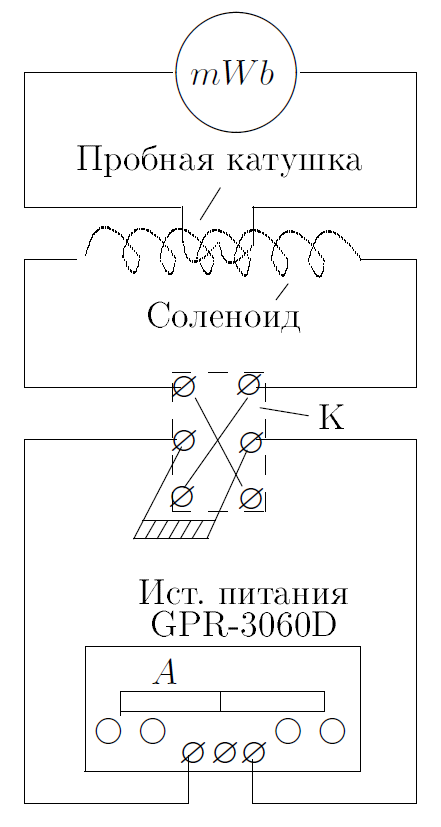
\includegraphics[width = 0.2\textwidth]{1.png}
  \end{center}
  \textbf{\caption{Схема установки.}}
\end{wrapfigure}
Основной частью установки является электронный осциллограф, трубка которого вынута и установлена в длинном соленоиде, создающим магнитное поле. Напряжение на отклоняющие пластины и питание подводятся к трубке многожильным кабелем.

Пучок электронов, вылетающих из катода с разными скоростями, ускоряется анодным напряжением. Пропустив пучок сквозь две узкие диафрагмы, можно выделить электроны с практически одинаковой продольной скоростью. Небольшое переменное напряжение, поступающее с клеммы "Контрольный сигнал" осциллографа на отклоняющие пластины, изменяет только поперечную составляющую скорости. При увеличении магнитного поля линия на экране стягивается в точку, а затем снова удлиняется. 

Магнитное поле создается постоянным током, величина которого регулируется ручками источника питания и измеряется амперметром. Ключ служит для изменения направления поля в соленоиде.

Величина магнитного поля определяется с помощью милливеберметра.

На точность результатов может влиять внешнее магнитное поле, особенно продольное. 

Измерения магнитного поля с помощью милливеберметра обычно проводятся в предварительных опыта: при отключении ключа устанавливается связь между силой тока и индукцией магнитного поля в соленоиде. 
\subsection*{Ход работы.}
Занесем в таблицу некоторые данные установки.
\begin{center}
\begin{tabular}{|c|c|c|}
\hline
Величина & Значение & $\sigma$ \\ \hline
$V$, кВ & 0,88 & 0,01 \\ \hline
$l$, м & 0,265 & 0,001 \\ \hline
$SN$, м$^2$ & 0,3 & 0,1 \\ \hline
\end{tabular}\\
\textbf{Таблица 1.} Некоторые параметры установки.
\end{center}
Для начала стоит определить связь между индукцией $B$ магнитного поля в соленоиде и током $I$ через обмотки магнита. Для этого снимем зависимость магнитного потока $\Phi = BSN$.
  \begin{center}
  \begin{tabular}{|c|c|c|c|}
\hline
$I$, A & $\sigma_I$, А & $\Phi$, мВб & $\sigma_{\Phi}$, мВб \\ \hline
0,26 & 0,01 & 0,35 & 0,01 \\ \hline
0,41 & 0,01 & 0,50 & 0,01 \\ \hline
0,79 & 0,01 & 1,05 & 0,01 \\ \hline
1,01 & 0,01 & 1,35 & 0,01 \\ \hline
1,49 & 0,01 & 1,95 & 0,01 \\ \hline
2,28 & 0,01 & 3,00 & 0,01 \\ \hline
2,54 & 0,01 & 3,30 & 0,01 \\ \hline
3,06 & 0,01 & 3,90 & 0,01 \\ \hline
3,64 & 0,01 & 4,50 & 0,01 \\ \hline
\end{tabular}\\
  \textbf{Таблица 2.} Зависимость $\Phi (I)$ в прямом направлении.\\
  \end{center}
  \begin{center}
    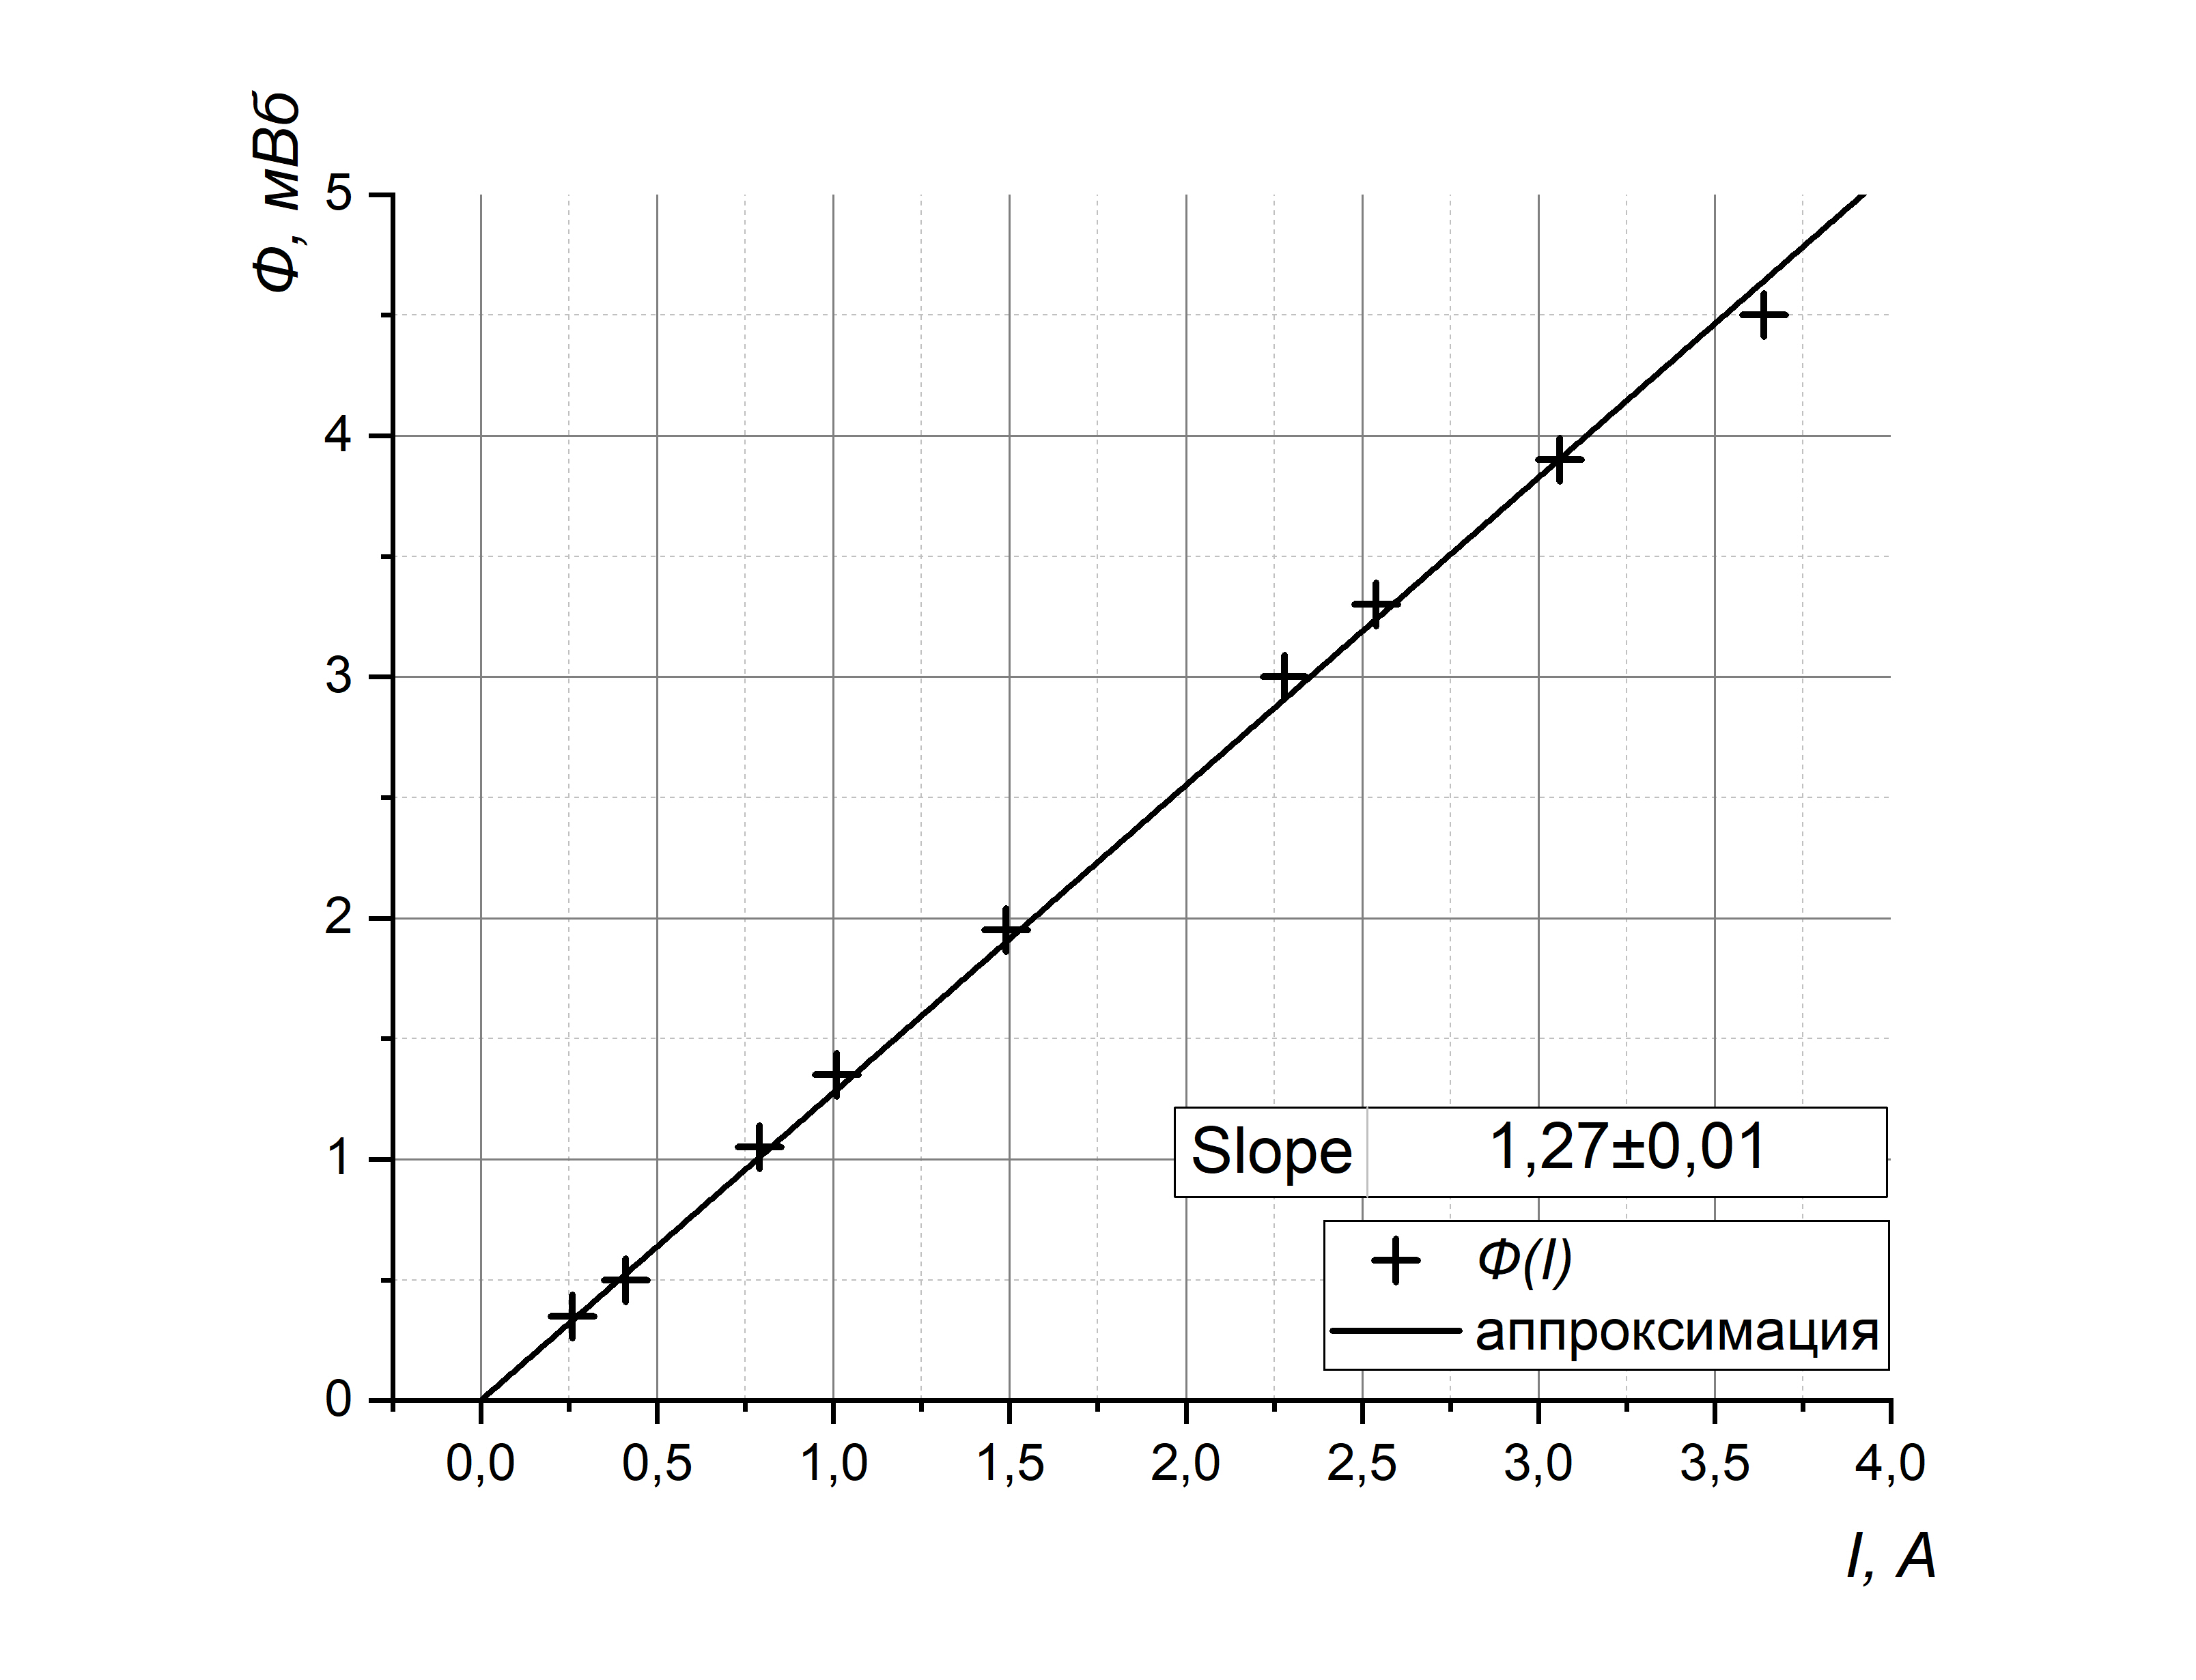
\includegraphics[width = 0.7\textwidth]{2.jpg}\\
  \textbf{График 1.} $\Phi (I)$ в прямом направлении.
  \end{center}
  \begin{center}
\begin{tabular}{|c|c|c|c|}
\hline
$I$, A & $\sigma_I$, А & $\Phi$, мВб & $\sigma_{\Phi}$, мВб \\ \hline
0,26 & 0,01 & 4,66 & 0,01 \\ \hline
0,41 & 0,01 & 4,47 & 0,01 \\ \hline
0,79 & 0,01 & 3,98 & 0,01 \\ \hline
1,01 & 0,01 & 3,69 & 0,01 \\ \hline
1,49 & 0,01 & 3,07 & 0,01 \\ \hline
2,28 & 0,01 & 2,05 & 0,01 \\ \hline
2,54 & 0,01 & 1,71 & 0,01 \\ \hline
3,06 & 0,01 & 1,03 & 0,01 \\ \hline
3,64 & 0,01 & 0,28 & 0,01 \\ \hline
\end{tabular}\\
\textbf{Таблица 3.} Зависимость $\Phi (I)$ в обратном направлении.
  \end{center} 
 \begin{center}
    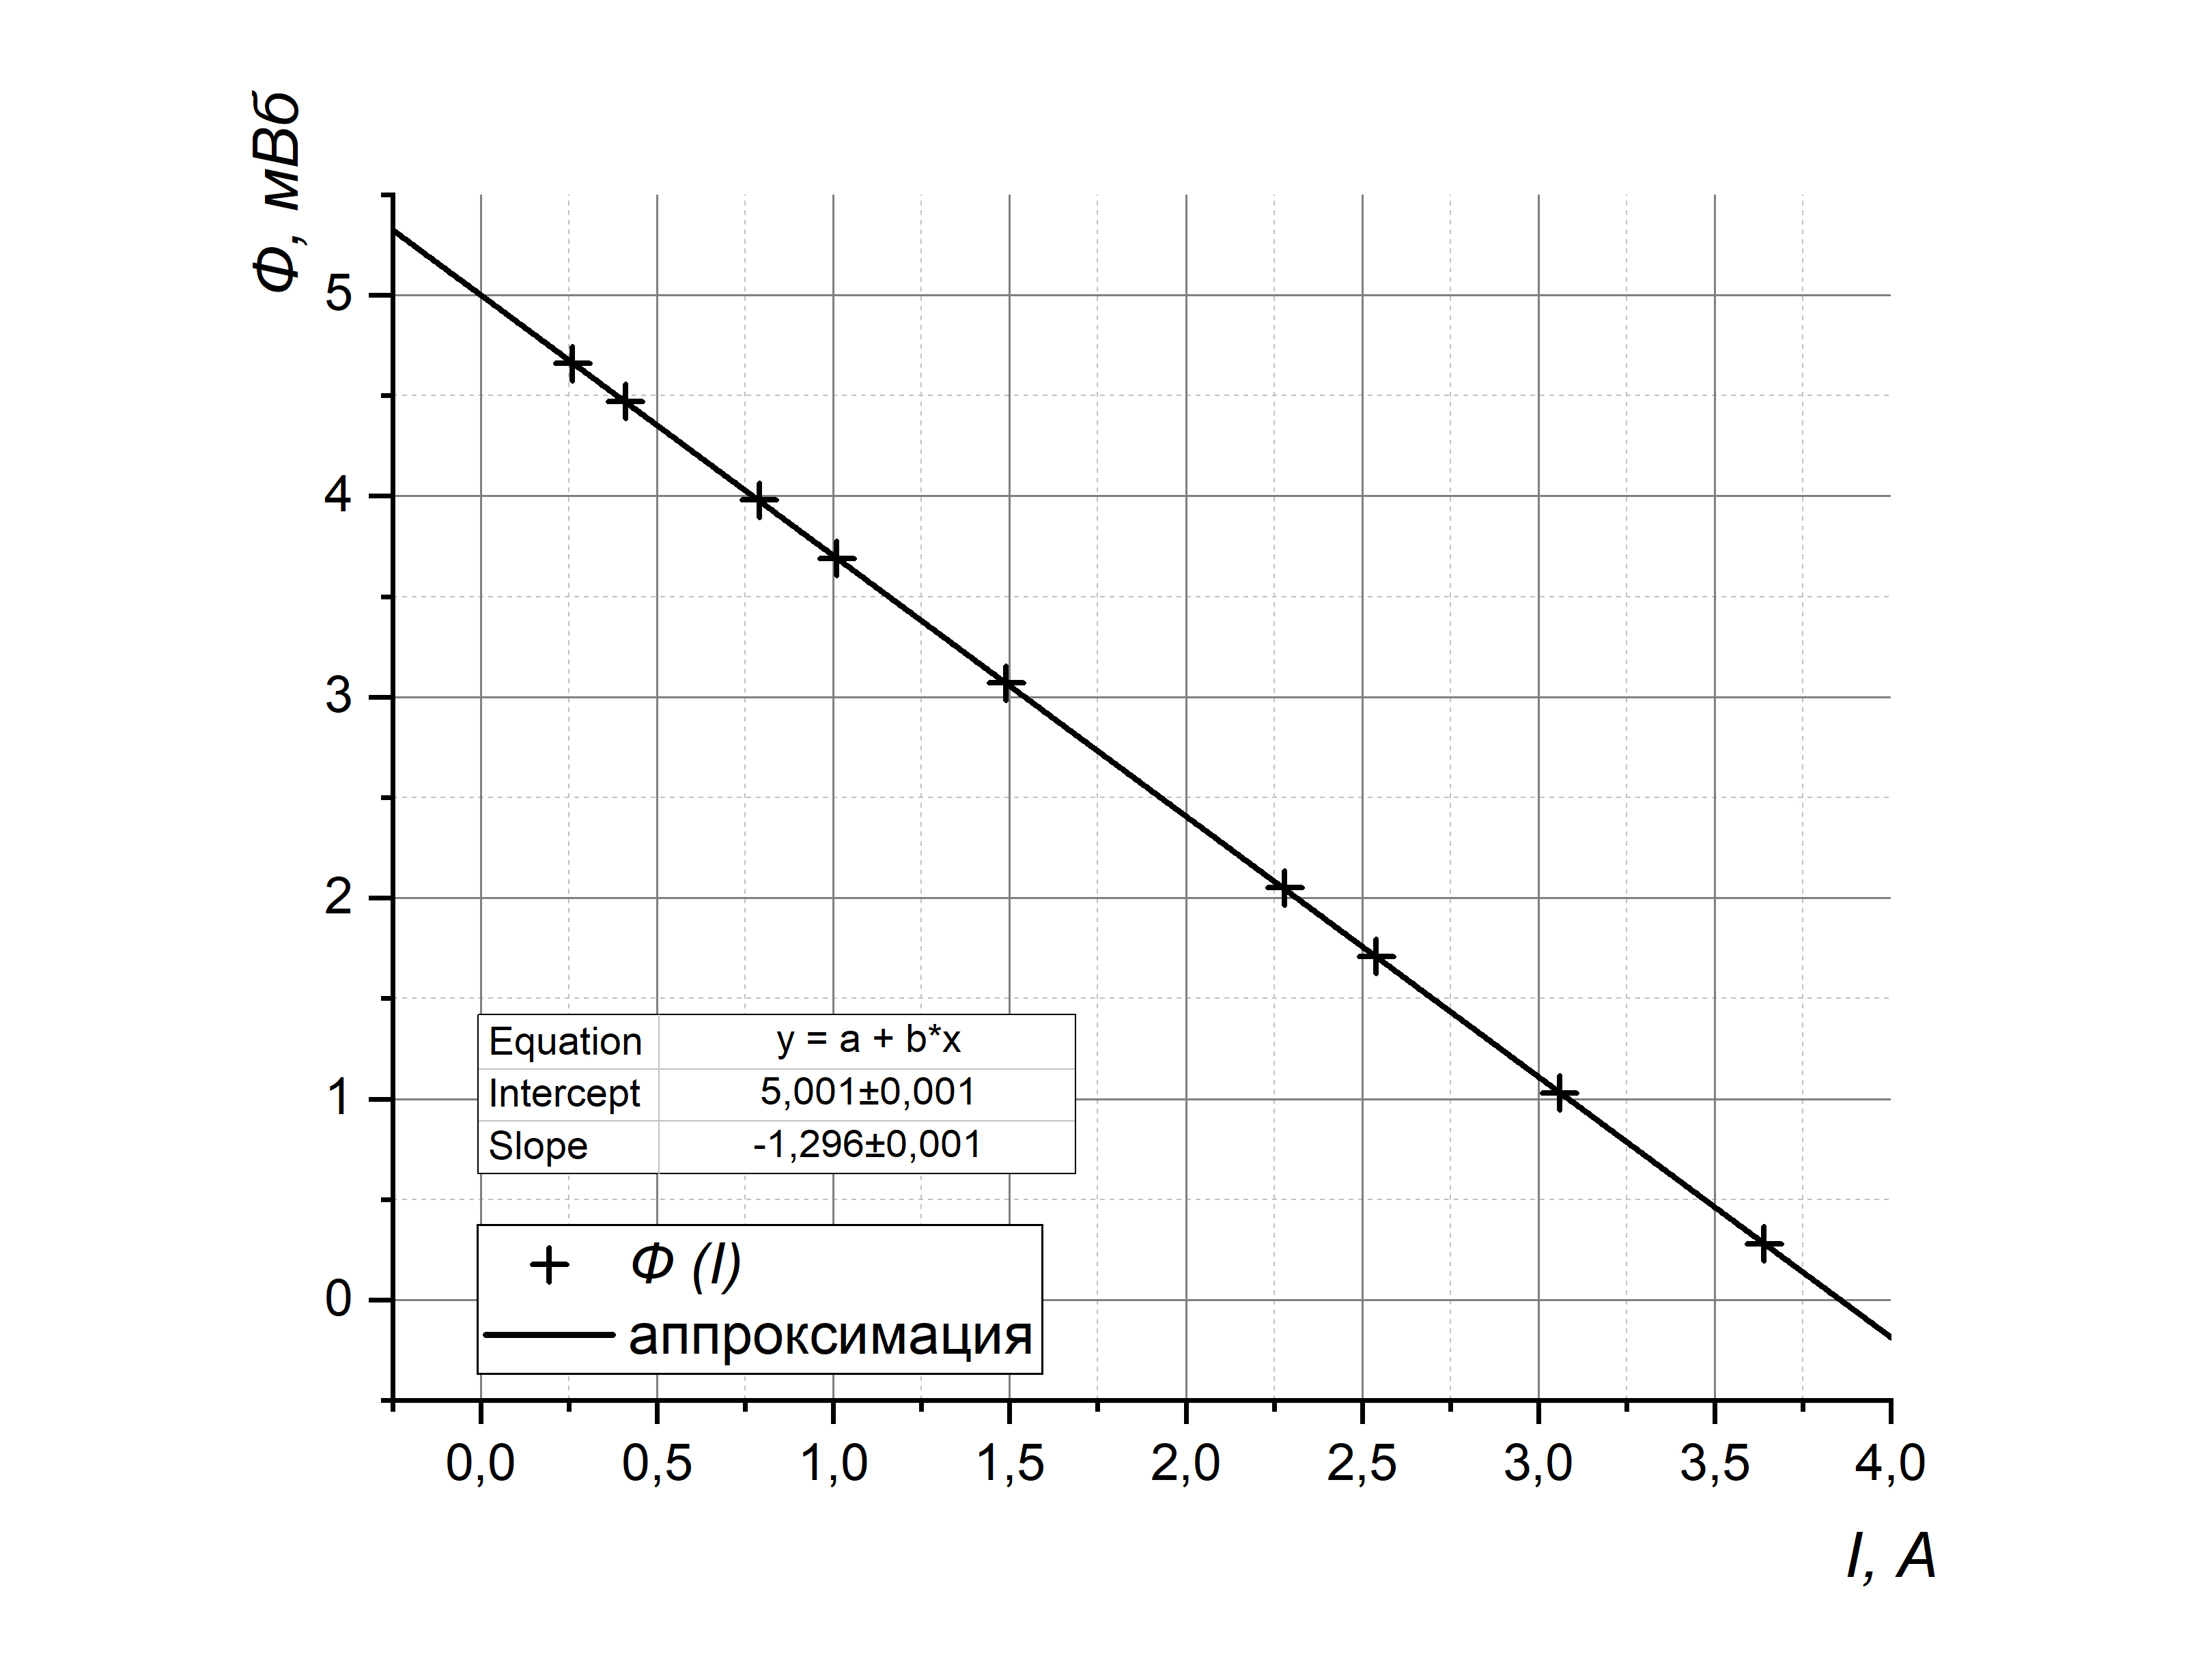
\includegraphics[width = 0.7\textwidth]{4.jpg}\\
  \textbf{График 2.} $\Phi (I)$ в обратном направлении.
  \end{center}
Теперь будем увеличивать постепенно ток и найдем ток при каждом фокусе, так как мы знаем зависимость $\Phi = \Phi(I)$ для каждого направления, то мы можем определить зависимость $B_{\Phi} = f(n)$.
\begin{center}
\begin{tabular}{|c|c|c|c|c|c|c|c|c|c|}
\hline
\multicolumn{5}{|c|}{В прямом направлении} & \multicolumn{5}{c|}{В обратном направлении} \\ \hline
n & $I_{\Phi}$, A & $\sigma_{I_{\Phi}}$, A & $B_{\Phi}$, мТл & $\sigma_{B_{\Phi}}$, мТл & n & $I_{\Phi}$, A & $\sigma_{I_{\Phi}}$, A & $B_{\Phi}$, мТл & $\sigma_{B_{\Phi}}$, мТл \\ \hline
1 & 0,53 & 0,01 & 2,24 & 0,02 & 1 & 0,58 & 0,01 & 14,2 & 0,1 \\ \hline
2 & 1,12 & 0,01 & 4,74 & 0,05 & 2 & 1,15 & 0,01 & 11,7 & 0,1 \\ \hline
3 & 1,7 & 0,01 & 7,2 & 0,1 & 3 & 1,78 & 0,01 & 8,9 & 0,1 \\ \hline
4 & 2,34 & 0,01 & 9,9 & 0,1 & 4 & 2,36 & 0,01 & 6,5 & 0,1 \\ \hline
5 & 2,89 & 0,01 & 12,2 & 0,1 & 5 & 2,86 & 0,01 & 4,31 & 0,04 \\ \hline
\end{tabular}\\
\textbf{Таблица 4.} Зависимость $B_{\Phi} = f(I)$.
\end{center}
\begin{center}
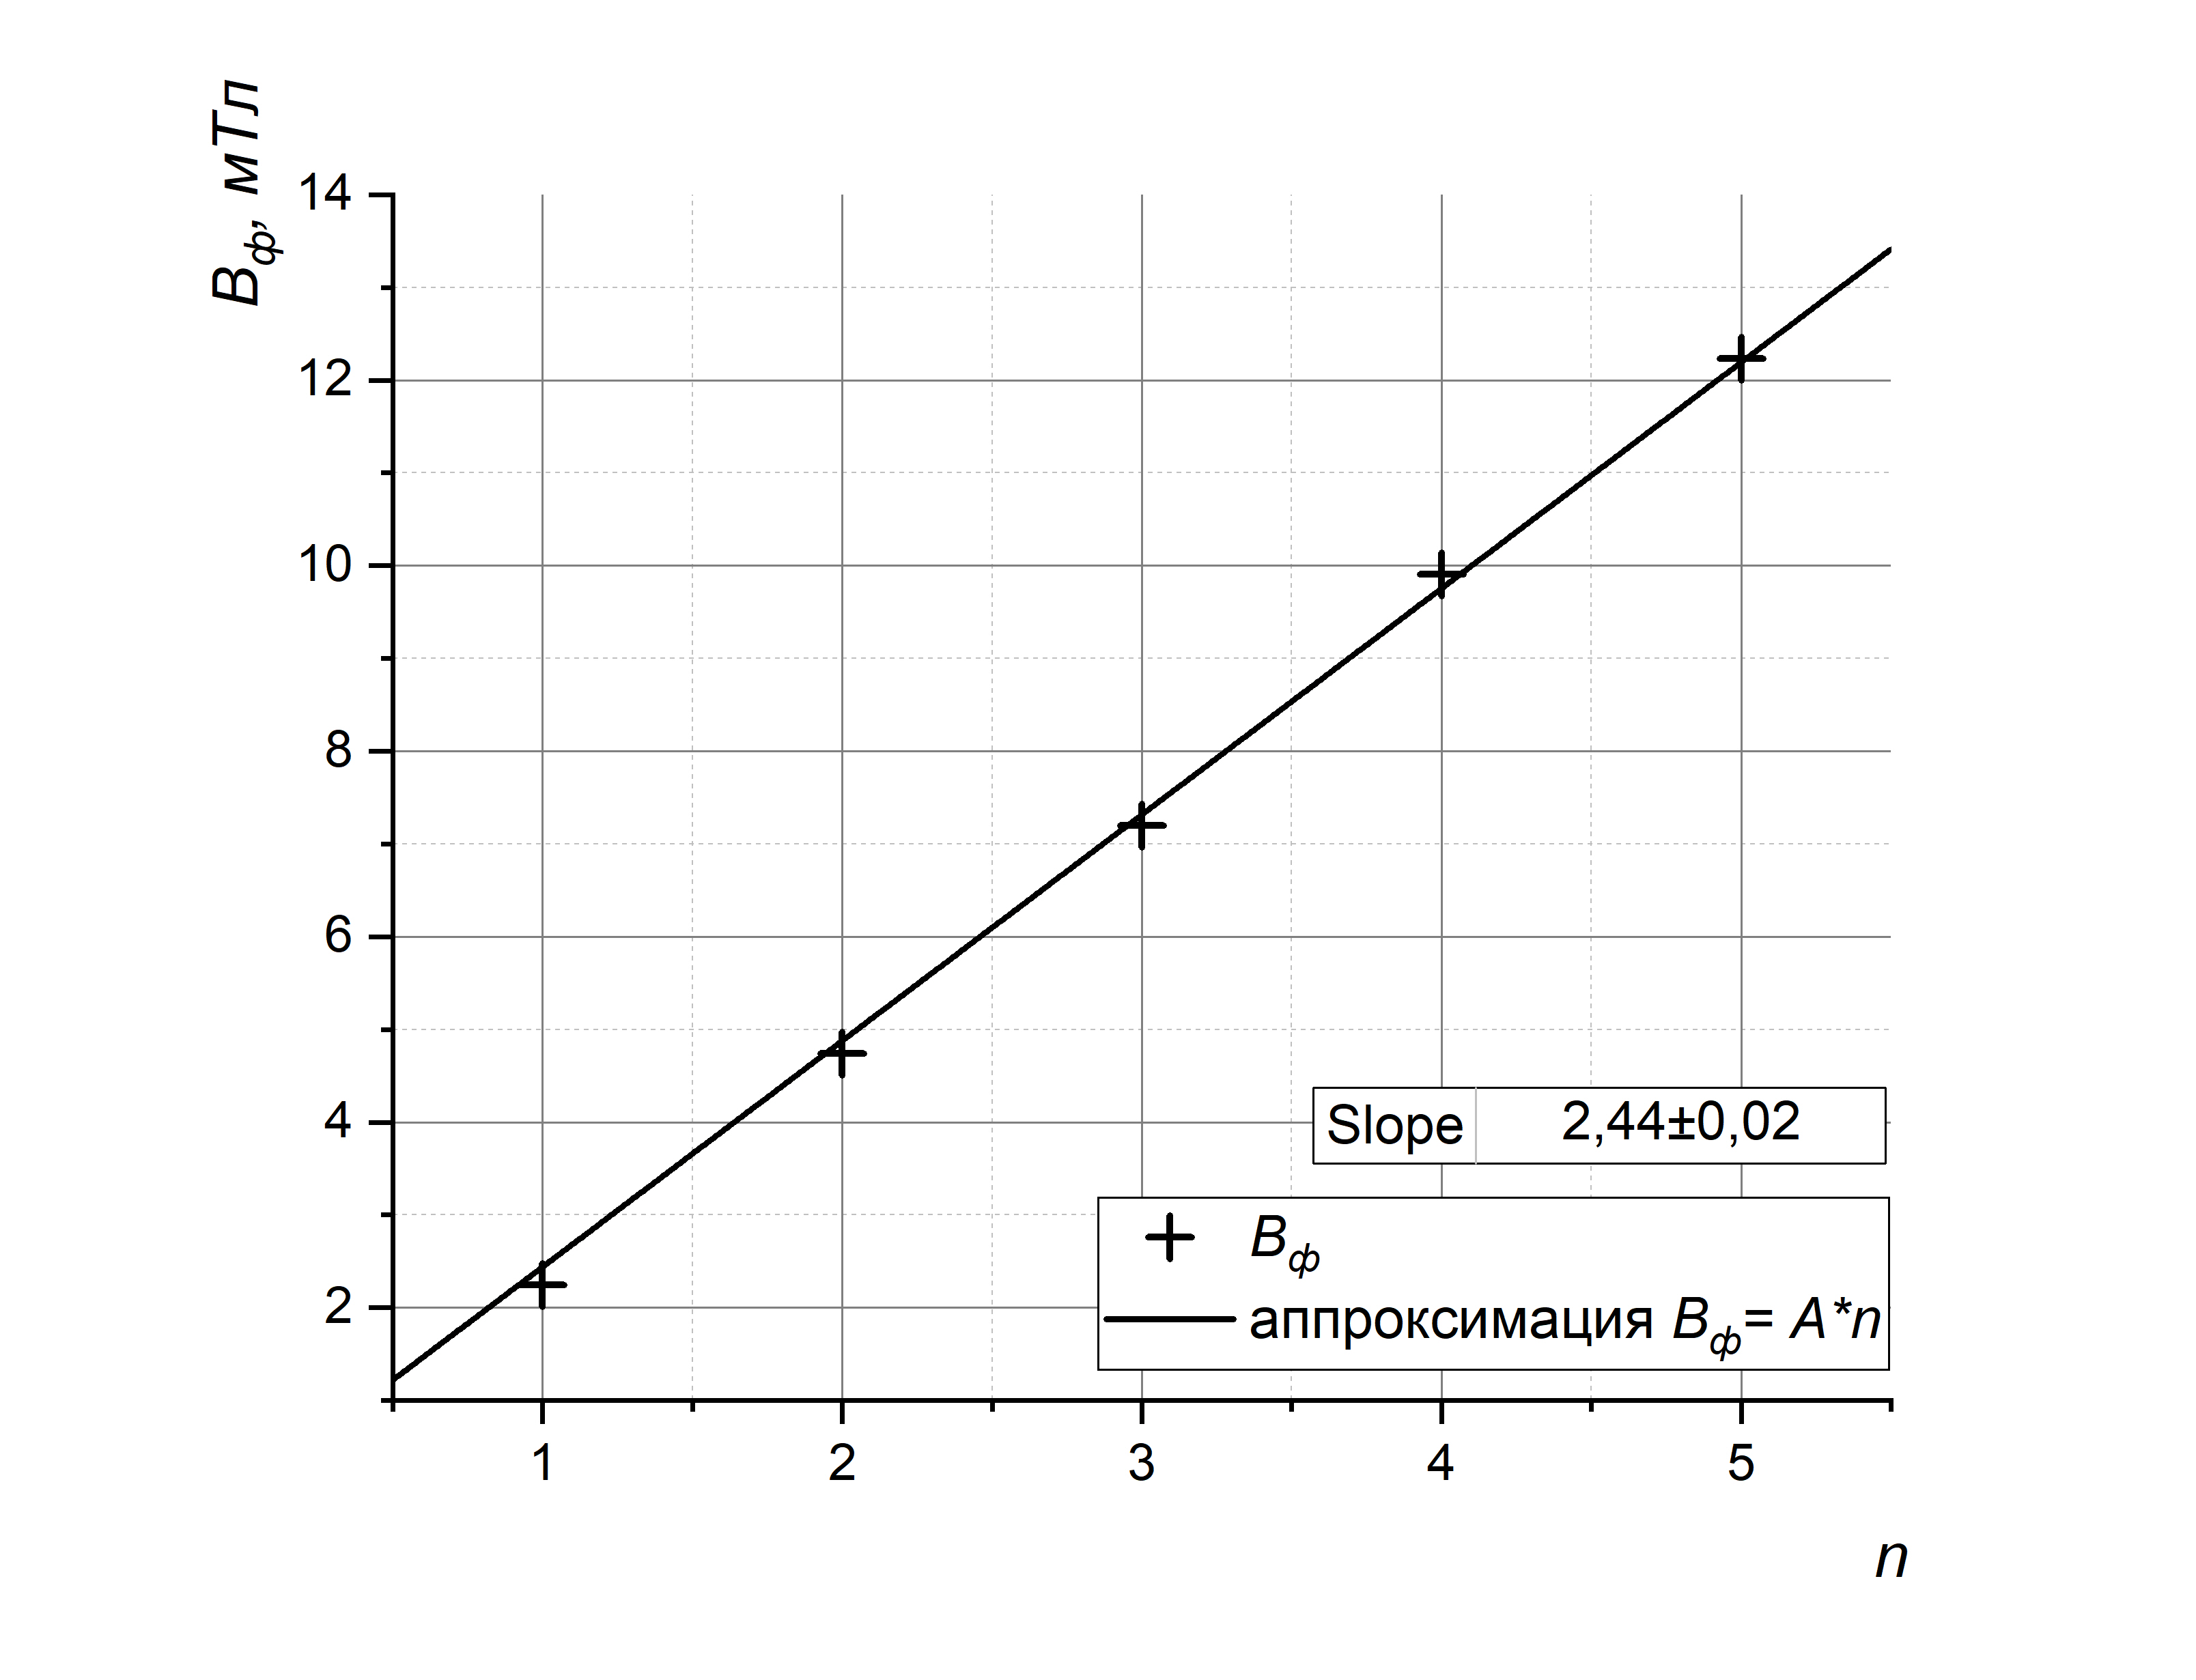
\includegraphics[width = 0.8\textwidth]{3.jpg}\\
\textbf{График 3.} $B_{\Phi} = f(I)$ в прямом направлении.
\end{center}
\begin{center}
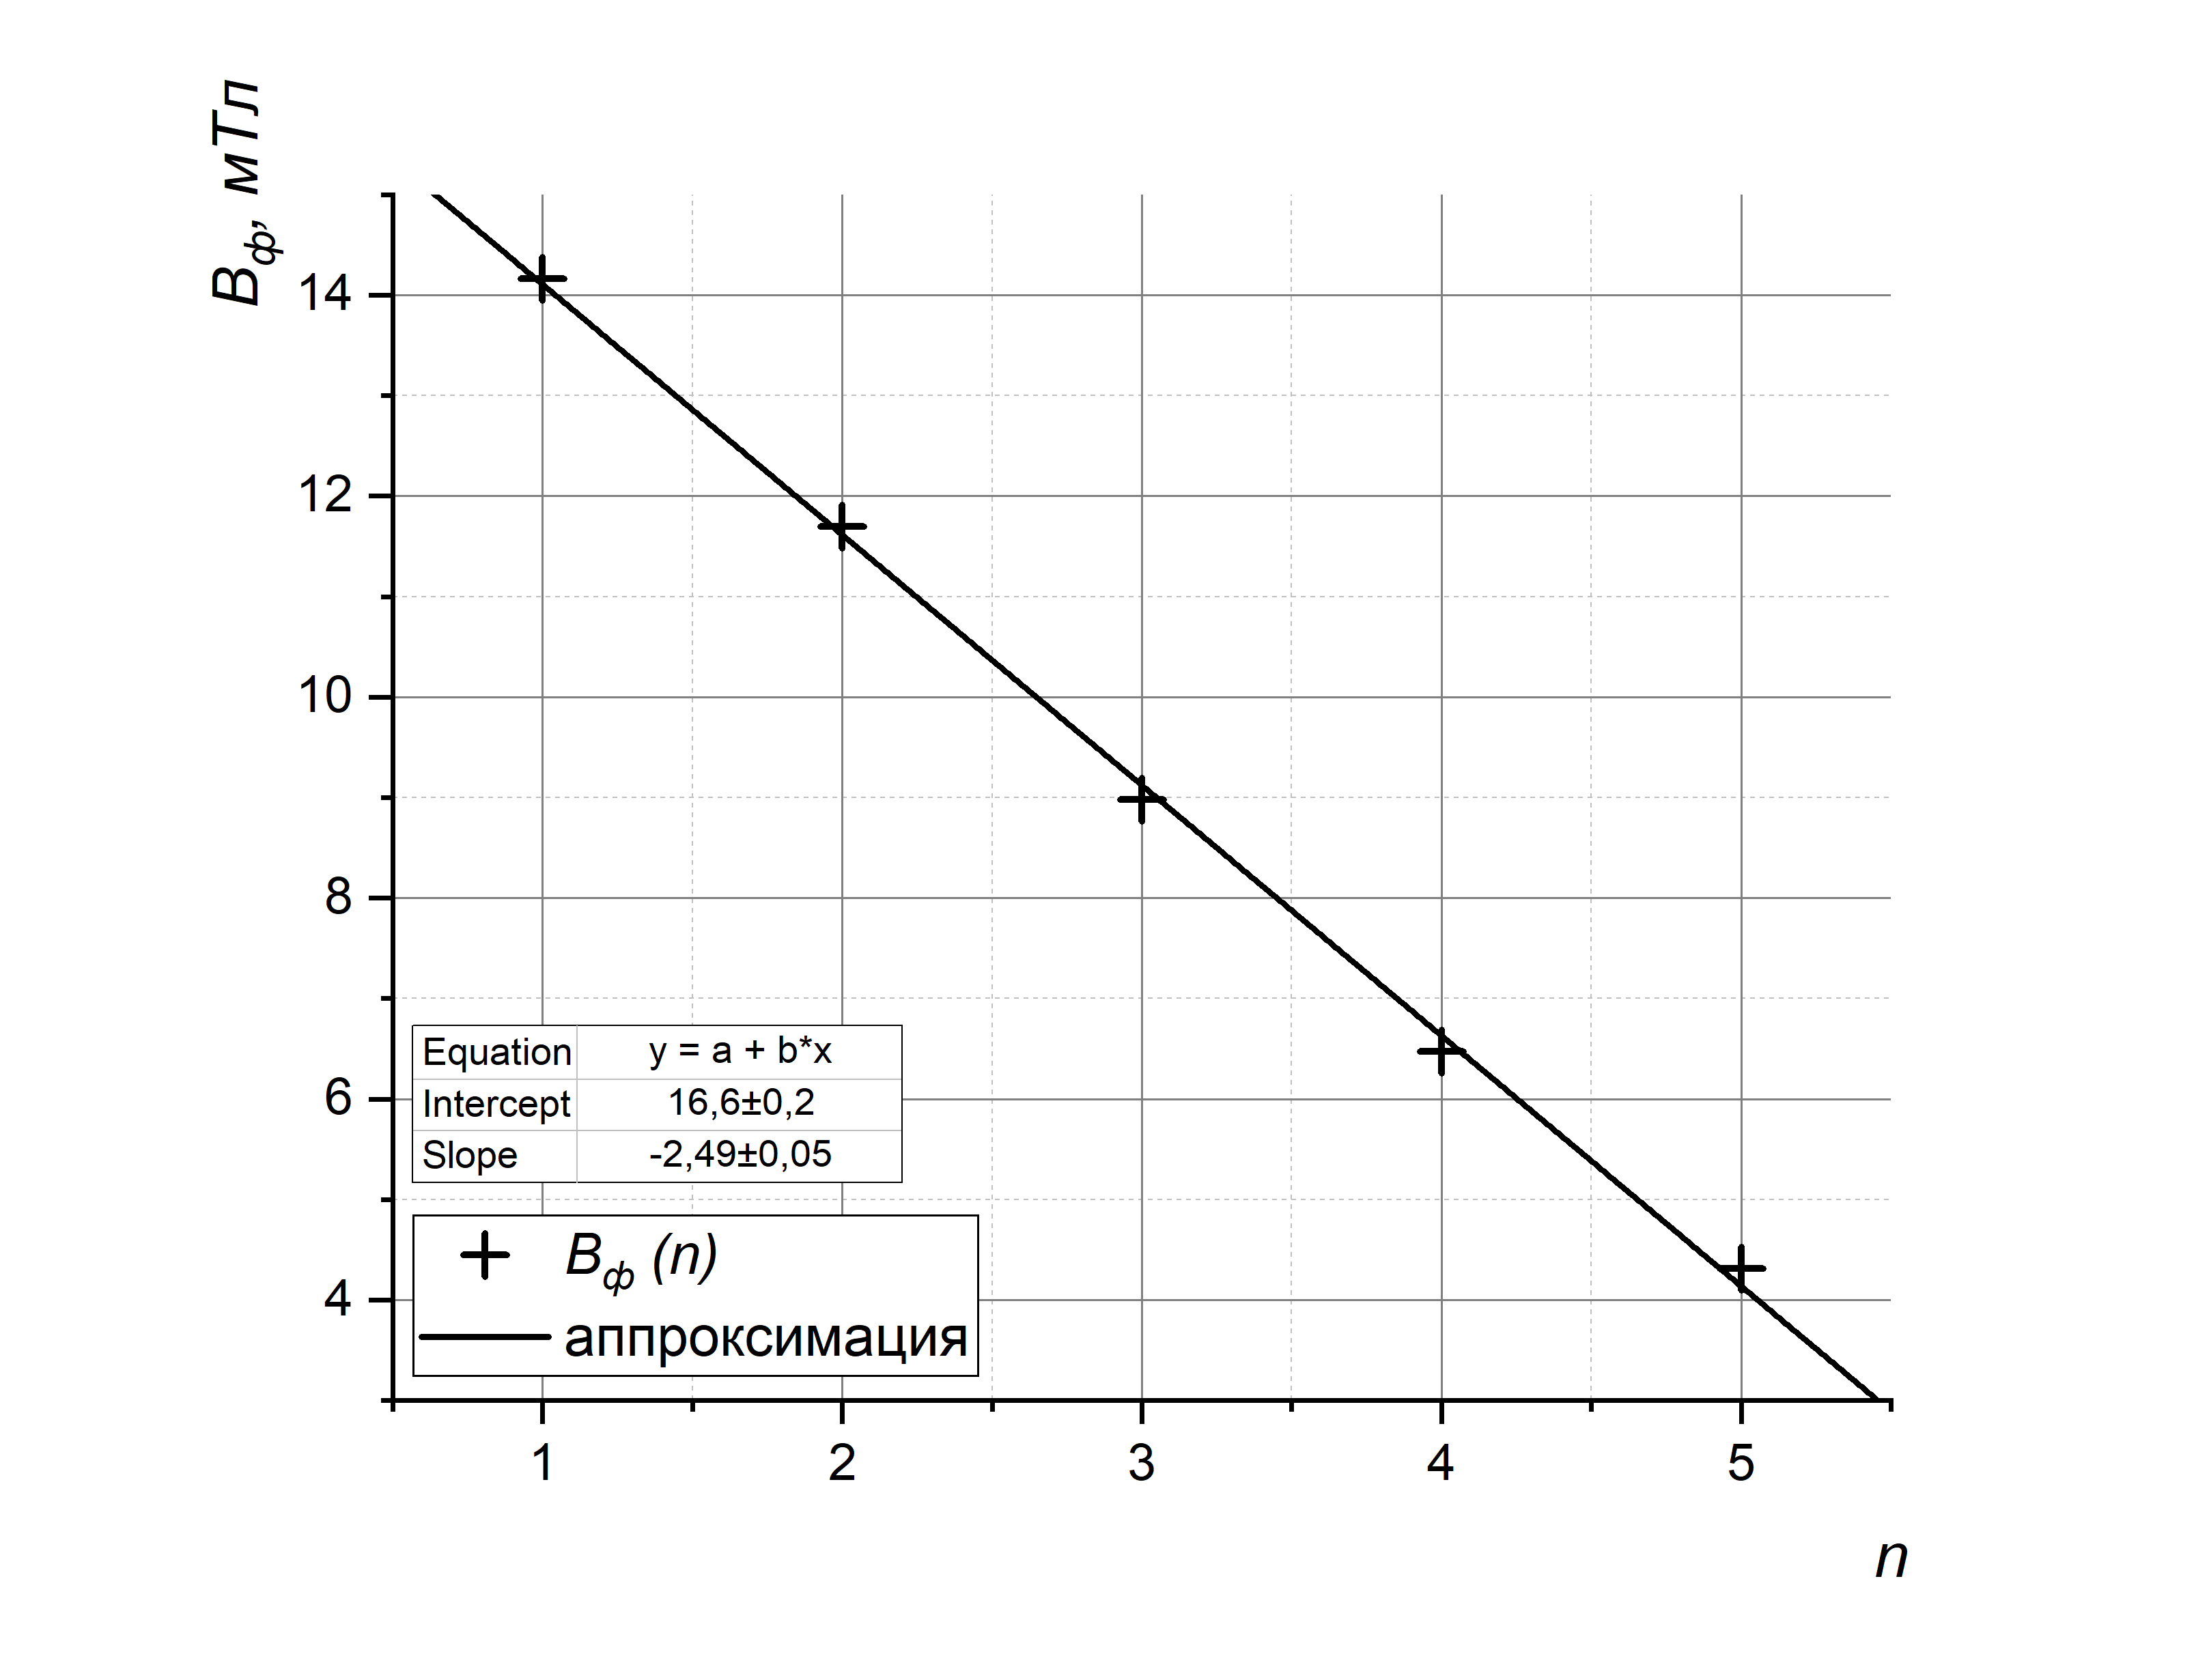
\includegraphics[width = 0.8\textwidth]{5.jpg}\\
\textbf{График 4.} $B_{\Phi} = f(I)$ в обратном направлении.
\end{center}
В итоге, подставив в формулу $(1)$ мы получаем, что 
\[\dfrac{e}{m} = \left(1,6 \pm 0,2\right) \cdot 10^{11} \text{Кл}/\text{кг}\]
Это значение очень близко к реальному $e/m = 1,76 \cdot 10^{11} \text{Кл}/\text{кг}$
\section*{B. Метод магнетрона.}
\subsection*{Цель работы}
Исследование зависимости анодного тока от тока, протекающего через соленоид при различных напряжениях на аноде лампы и по результатам измерений рассчитать удельный заряд электрона $e/m$.
\subsection*{В работе используются.}
Электронная лампа с цилиндрическим анодом; соленоид; источники питания лампы и соленоида; вольтметр постоянного тока; миллиамперметр, амперметр.
\subsection*{Теоретическая справка.}
Здесь удельный заряд электрона определяется по формуле
\begin{equation}
\dfrac{e}{m_e} = \dfrac{8V_a}{B_{\text{кр}}^2r_a^2},
\end{equation}
где $V_a$ - анодное напряжение, $B_{\text{кр}}$ - критическое поле, $r_a$ - радиус анода.
\subsection*{Описание установки.}
\begin{wrapfigure}{l}{0.3\textwidth}
  \begin{center}
    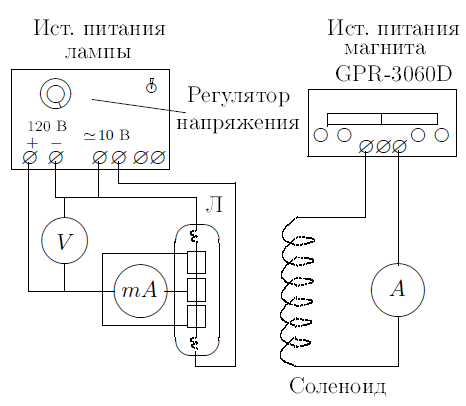
\includegraphics[width = 0.3\textwidth]{6.png}
  \end{center}
  \textbf{\caption{Схема установки.}}
\end{wrapfigure}
Два крайних цилиндра изолированы от среднего небольшими зазорами и используются для устранения краевых эффектов на торцах среднего цилиндра, ток с которого используется при измерениях. В качестве катода используется тонкая вольфрамовая проволока. Катод разогревается переменным током, отбираемым от стабилизированного источника питания. 

С этого же источника на анод лампы подается напряжение, регулируемое с помощью потенциометра и измеряемое вольтметром.

Индукция магнитного поля в соленоиде рассчитывается по току $I_m$, протекающему через обмотку соленоида. Коэффициент пропорциональности между ними указан в установке.

Лампа закреплена в соленоиде. Магнитное поле в соленоиде создается постоянным током, сила которого регулируется ручками источника питания и измеряется амперметром.
\newpage
\subsection*{Ход работы.}
Запишем некоторые параметры установки в таблицу
\begin{center}
\begin{tabular}{|c|c|c|}
\hline
Величина & Значение & $\sigma$ \\ \hline
$K$, Тл/A & $2,8 \cdot 10^{-2}$ & $10^{-4}$ \\ \hline
$r_a$, мм & 12 & 0,1 \\ \hline
\end{tabular}\\
\textbf{Таблица 5.} Параметры установки.
\end{center}
Снимем зависимость анодного тока от тока через соленоид для различных значений $V_a$.
\begin{center}
\begin{tabular}{|c|c|c|c|c|c|}
\hline
$I_m$, мА & $\sigma_{I_m}$, мА & $B$, мТл & $\sigma_B$, мТл & $I_a$, мкА & $\sigma_{I_a}$, мкА \\ \hline
0 & 4 & 0,0 & 0,1 & 266 & 2 \\ \hline
20 & 4 & 0,6 & 0,1 & 270 & 2 \\ \hline
32 & 4 & 0,9 & 0,1 & 266 & 2 \\ \hline
36 & 4 & 1,0 & 0,1 & 266 & 2 \\ \hline
44 & 4 & 1,2 & 0,1 & 266 & 2 \\ \hline
60 & 4 & 1,7 & 0,1 & 266 & 2 \\ \hline
76 & 4 & 2,1 & 0,1 & 262 & 2 \\ \hline
88 & 4 & 2,5 & 0,1 & 256 & 2 \\ \hline
96 & 4 & 2,7 & 0,1 & 252 & 2 \\ \hline
100 & 4 & 2,8 & 0,1 & 242 & 2 \\ \hline
108 & 4 & 3,0 & 0,1 & 236 & 2 \\ \hline
116 & 4 & 3,2 & 0,1 & 232 & 2 \\ \hline
124 & 4 & 3,5 & 0,1 & 230 & 2 \\ \hline
132 & 4 & 3,7 & 0,1 & 232 & 2 \\ \hline
136 & 4 & 3,8 & 0,1 & 222 & 2 \\ \hline
144 & 4 & 4,0 & 0,1 & 206 & 2 \\ \hline
148 & 4 & 4,1 & 0,1 & 200 & 2 \\ \hline
156 & 4 & 4,4 & 0,1 & 186 & 2 \\ \hline
160 & 4 & 4,5 & 0,1 & 180 & 2 \\ \hline
168 & 4 & 4,7 & 0,1 & 164 & 2 \\ \hline
176 & 4 & 4,9 & 0,1 & 140 & 2 \\ \hline
182 & 4 & 5,1 & 0,1 & 104 & 2 \\ \hline
184 & 4 & 5,2 & 0,1 & 88 & 2 \\ \hline
188 & 4 & 5,3 & 0,1 & 56 & 2 \\ \hline
190 & 4 & 5,3 & 0,1 & 40 & 2 \\ \hline
194 & 4 & 5,4 & 0,1 & 28 & 2 \\ \hline
202 & 4 & 5,7 & 0,1 & 18 & 2 \\ \hline
208 & 4 & 5,8 & 0,1 & 12 & 2 \\ \hline
216 & 4 & 6,0 & 0,1 & 10 & 2 \\ \hline
224 & 4 & 6,3 & 0,1 & 6 & 2 \\ \hline
236 & 4 & 6,6 & 0,1 & 4 & 2 \\ \hline
244 & 4 & 6,8 & 0,1 & 3 & 2 \\ \hline
256 & 4 & 7,2 & 0,1 & 2 & 2 \\ \hline
284 & 4 & 8,0 & 0,1 & 0 & 2 \\ \hline
\end{tabular}\\
\textbf{Таблица 6.} Зависимость $I_a(B)$ для $V_a = (70 \pm 1)$ В.
\end{center}
\begin{center}
\begin{tabular}{|c|c|c|c|c|c|}
\hline
$I_m$, мА & $\sigma_{I_m}$, мА & $B$, мТл & $\sigma_B$, мТл & $I_a$, мкА & $\sigma_{I_a}$, мкА \\ \hline
0 & 4 & 0,0 & 0,1 & 254 & 2 \\ \hline
8 & 4 & 0,2 & 0,1 & 258 & 2 \\ \hline
36 & 4 & 1,0 & 0,1 & 254 & 2 \\ \hline
48 & 4 & 1,3 & 0,1 & 254 & 2 \\ \hline
60 & 4 & 1,7 & 0,1 & 254 & 2 \\ \hline
76 & 4 & 2,1 & 0,1 & 254 & 2 \\ \hline
84 & 4 & 2,4 & 0,1 & 252 & 2 \\ \hline
92 & 4 & 2,6 & 0,1 & 250 & 2 \\ \hline
104 & 4 & 2,9 & 0,1 & 238 & 2 \\ \hline
108 & 4 & 3,0 & 0,1 & 226 & 2 \\ \hline
116 & 4 & 3,2 & 0,1 & 220 & 2 \\ \hline
120 & 4 & 3,4 & 0,1 & 216 & 2 \\ \hline
128 & 4 & 3,6 & 0,1 & 214 & 2 \\ \hline
134 & 4 & 3,8 & 0,1 & 220 & 2 \\ \hline
140 & 4 & 3,9 & 0,1 & 220 & 2 \\ \hline
152 & 4 & 4,3 & 0,1 & 202 & 2 \\ \hline
158 & 4 & 4,4 & 0,1 & 200 & 2 \\ \hline
162 & 4 & 4,5 & 0,1 & 192 & 2 \\ \hline
170 & 4 & 4,8 & 0,1 & 184 & 2 \\ \hline
180 & 4 & 5,0 & 0,1 & 168 & 2 \\ \hline
192 & 4 & 5,4 & 0,1 & 120 & 2 \\ \hline
196 & 4 & 5,5 & 0,1 & 90 & 2 \\ \hline
204 & 4 & 5,7 & 0,1 & 50 & 2 \\ \hline
208 & 4 & 5,8 & 0,1 & 32 & 2 \\ \hline
212 & 4 & 5,9 & 0,1 & 24 & 2 \\ \hline
216 & 4 & 6,0 & 0,1 & 20 & 2 \\ \hline
224 & 4 & 6,3 & 0,1 & 14 & 2 \\ \hline
232 & 4 & 6,5 & 0,1 & 10 & 2 \\ \hline
242 & 4 & 6,8 & 0,1 & 6 & 2 \\ \hline
256 & 4 & 7,2 & 0,1 & 4 & 2 \\ \hline
268 & 4 & 7,5 & 0,1 & 3 & 2 \\ \hline
284 & 4 & 8,0 & 0,1 & 2 & 2 \\ \hline
300 & 4 & 8,4 & 0,1 & 0 & 2 \\ \hline
\end{tabular}\\
\textbf{Таблица 7.} Зависимость $I_a(B)$ для $V_a = (80 \pm 1)$ В.
\end{center}
\begin{center}
\begin{tabular}{|c|c|c|c|c|c|}
\hline
$I_m$, мА & $\sigma_{I_m}$, мА & $B$, мТл & $\sigma_B$, мТл & $I_a$, мкА & $\sigma_{I_a}$, мкА \\ \hline
0 & 4 & 0,0 & 0,1 & 262 & 2 \\ \hline
16 & 4 & 0,4 & 0,1 & 260 & 2 \\ \hline
44 & 4 & 1,2 & 0,1 & 258 & 2 \\ \hline
52 & 4 & 1,5 & 0,1 & 260 & 2 \\ \hline
68 & 4 & 1,9 & 0,1 & 260 & 2 \\ \hline
84 & 4 & 2,4 & 0,1 & 260 & 2 \\ \hline
104 & 4 & 2,9 & 0,1 & 256 & 2 \\ \hline
112 & 4 & 3,1 & 0,1 & 240 & 2 \\ \hline
116 & 4 & 3,2 & 0,1 & 234 & 2 \\ \hline
120 & 4 & 3,4 & 0,1 & 226 & 2 \\ \hline
128 & 4 & 3,6 & 0,1 & 226 & 2 \\ \hline
140 & 4 & 3,9 & 0,1 & 218 & 2 \\ \hline
144 & 4 & 4,0 & 0,1 & 208 & 2 \\ \hline
152 & 4 & 4,3 & 0,1 & 230 & 2 \\ \hline
164 & 4 & 4,6 & 0,1 & 220 & 2 \\ \hline
174 & 4 & 4,9 & 0,1 & 198 & 2 \\ \hline
180 & 4 & 5,0 & 0,1 & 190 & 2 \\ \hline
186 & 4 & 5,2 & 0,1 & 184 & 2 \\ \hline
190 & 4 & 5,3 & 0,1 & 180 & 2 \\ \hline
196 & 4 & 5,5 & 0,1 & 166 & 2 \\ \hline
200 & 4 & 5,6 & 0,1 & 158 & 2 \\ \hline
204 & 4 & 5,7 & 0,1 & 142 & 2 \\ \hline
208 & 4 & 5,8 & 0,1 & 108 & 2 \\ \hline
212 & 4 & 5,9 & 0,1 & 84 & 2 \\ \hline
216 & 4 & 6,0 & 0,1 & 54 & 2 \\ \hline
222 & 4 & 6,2 & 0,1 & 34 & 2 \\ \hline
228 & 4 & 6,4 & 0,1 & 24 & 2 \\ \hline
234 & 4 & 6,6 & 0,1 & 18 & 2 \\ \hline
240 & 4 & 6,7 & 0,1 & 12 & 2 \\ \hline
248 & 4 & 6,9 & 0,1 & 10 & 2 \\ \hline
264 & 4 & 7,4 & 0,1 & 6 & 2 \\ \hline
278 & 4 & 7,8 & 0,1 & 4 & 2 \\ \hline
288 & 4 & 8,1 & 0,1 & 2 & 2 \\ \hline
300 & 4 & 8,4 & 0,1 & 1 & 2 \\ \hline
312 & 4 & 8,7 & 0,1 & 0 & 2 \\ \hline
\end{tabular}\\
\textbf{Таблица 8.} Зависимость $I_a(B)$ для $V_a = (90 \pm 1)$ В.
\end{center}
\begin{center}
\begin{tabular}{|c|c|c|c|c|c|}
\hline
$I_m$, мА & $\sigma_{I_m}$, мА & $B$, мТл & $\sigma_B$, мТл & $I_a$, мкА & $\sigma_{I_a}$, мкА \\ \hline
0 & 4 & 0,0 & 0,1 & 264 & 2 \\ \hline
14 & 4 & 0,4 & 0,1 & 266 & 2 \\ \hline
40 & 4 & 1,1 & 0,1 & 264 & 2 \\ \hline
64 & 4 & 1,8 & 0,1 & 266 & 2 \\ \hline
72 & 4 & 2,0 & 0,1 & 268 & 2 \\ \hline
80 & 4 & 2,2 & 0,1 & 268 & 2 \\ \hline
96 & 4 & 2,7 & 0,1 & 264 & 2\\ \hline
108 & 4 & 3,0 & 0,1 & 264 & 2 \\ \hline
120 & 4 & 3,4 & 0,1 & 250 & 2 \\ \hline
130 & 4 & 3,6 & 0,1 & 238 & 2 \\ \hline
144 & 4 & 4,0 & 0,1 & 232 & 2 \\ \hline
156 & 4 & 4,4 & 0,1 & 248 & 2 \\ \hline
164 & 4 & 4,6 & 0,1 & 242 & 2 \\ \hline
168 & 4 & 4,7 & 0,1 & 236 & 2 \\ \hline
180 & 4 & 5,0 & 0,1 & 214 & 2 \\ \hline
192 & 4 & 5,4 & 0,1 & 204 & 2 \\ \hline
200 & 4 & 5,6 & 0,1 & 198 & 2 \\ \hline
208 & 4 & 5,8 & 0,1 & 178 & 2 \\ \hline
212 & 4 & 5,9 & 0,1 & 158 & 2 \\ \hline
216 & 4 & 6,0 & 0,1 & 150 & 2 \\ \hline
224 & 4 & 6,3 & 0,1 & 98 & 2 \\ \hline
230 & 4 & 6,4 & 0,1 & 50 & 2 \\ \hline
238 & 4 & 6,7 & 0,1 & 28 & 2 \\ \hline
248 & 4 & 6,9 & 0,1 & 20 & 2 \\ \hline
260 & 4 & 7,3 & 0,1 & 11 & 2 \\ \hline
272 & 4 & 7,6 & 0,1 & 8 & 2 \\ \hline
280 & 4 & 7,8 & 0,1 & 6 & 2 \\ \hline
292 & 4 & 8,2 & 0,1 & 4 & 2 \\ \hline
300 & 4 & 8,4 & 0,1 & 3 & 2 \\ \hline
\end{tabular}\\
\textbf{Таблица 9.} Зависимость $I_a(B)$ для $V_a = (100 \pm 1)$ В.
\end{center}
\begin{center}
\begin{tabular}{|c|c|c|c|c|c|}
\hline
$I_m$, мА & $\sigma_{I_m}$, мА & $B$, мТл & $\sigma_B$, мТл & $I_a$, мкА & $\sigma_{I_a}$, мкА \\ \hline
0 & 4 & 0,0 & 0,1 & 268 & 2 \\ \hline
20 & 4 & 0,6 & 0,1 & 270 & 2 \\ \hline
40 & 4 & 1,1 & 0,1 & 264 & 2 \\ \hline
54 & 4 & 1,5 & 0,1 & 266 & 2 \\ \hline
68 & 4 & 1,9 & 0,1 & 270 & 2 \\ \hline
88 & 4 & 2,5 & 0,1 & 268 & 2 \\ \hline
114 & 4 & 3,2 & 0,1 & 266 & 2 \\ \hline
140 & 4 & 3,9 & 0,1 & 244 & 2 \\ \hline
156 & 4 & 4,4 & 0,1 & 244 & 2 \\ \hline
168 & 4 & 4,7 & 0,1 & 254 & 2 \\ \hline
172 & 4 & 4,8 & 0,1 & 250 & 2 \\ \hline
180 & 4 & 5,0 & 0,1 & 242 & 2 \\ \hline
188 & 4 & 5,3 & 0,1 & 224 & 2 \\ \hline
196 & 4 & 5,5 & 0,1 & 214 & 2 \\ \hline
208 & 4 & 5,8 & 0,1 & 200 & 2 \\ \hline
212 & 4 & 5,9 & 0,1 & 200 & 2 \\ \hline
220 & 4 & 6,2 & 0,1 & 186 & 2 \\ \hline
224 & 4 & 6,3 & 0,1 & 166 & 2 \\ \hline
230 & 4 & 6,4 & 0,1 & 128 & 2 \\ \hline
236 & 4 & 6,6 & 0,1 & 88 & 2 \\ \hline
240 & 4 & 6,7 & 0,1 & 58 & 2 \\ \hline
244 & 4 & 6,8 & 0,1 & 40 & 2 \\ \hline
248 & 4 & 6,9 & 0,1 & 32 & 2 \\ \hline
256 & 4 & 7,2 & 0,1 & 22 & 2 \\ \hline
262 & 4 & 7,3 & 0,1 & 20 & 2 \\ \hline
268 & 4 & 7,5 & 0,1 & 14 & 2 \\ \hline
278 & 4 & 7,8 & 0,1 & 10 & 2 \\ \hline
284 & 4 & 8,0 & 0,1 & 8 & 2 \\ \hline
292 & 4 & 8,2 & 0,1 & 8 & 2 \\ \hline
\end{tabular}\\
\textbf{Таблица 10.} Зависимость $I_a(B)$ для $V_a = (110 \pm 1)$ В.
\end{center}
\newpage
Запишем данные из вышеприведенных таблиц в один график
\begin{center}
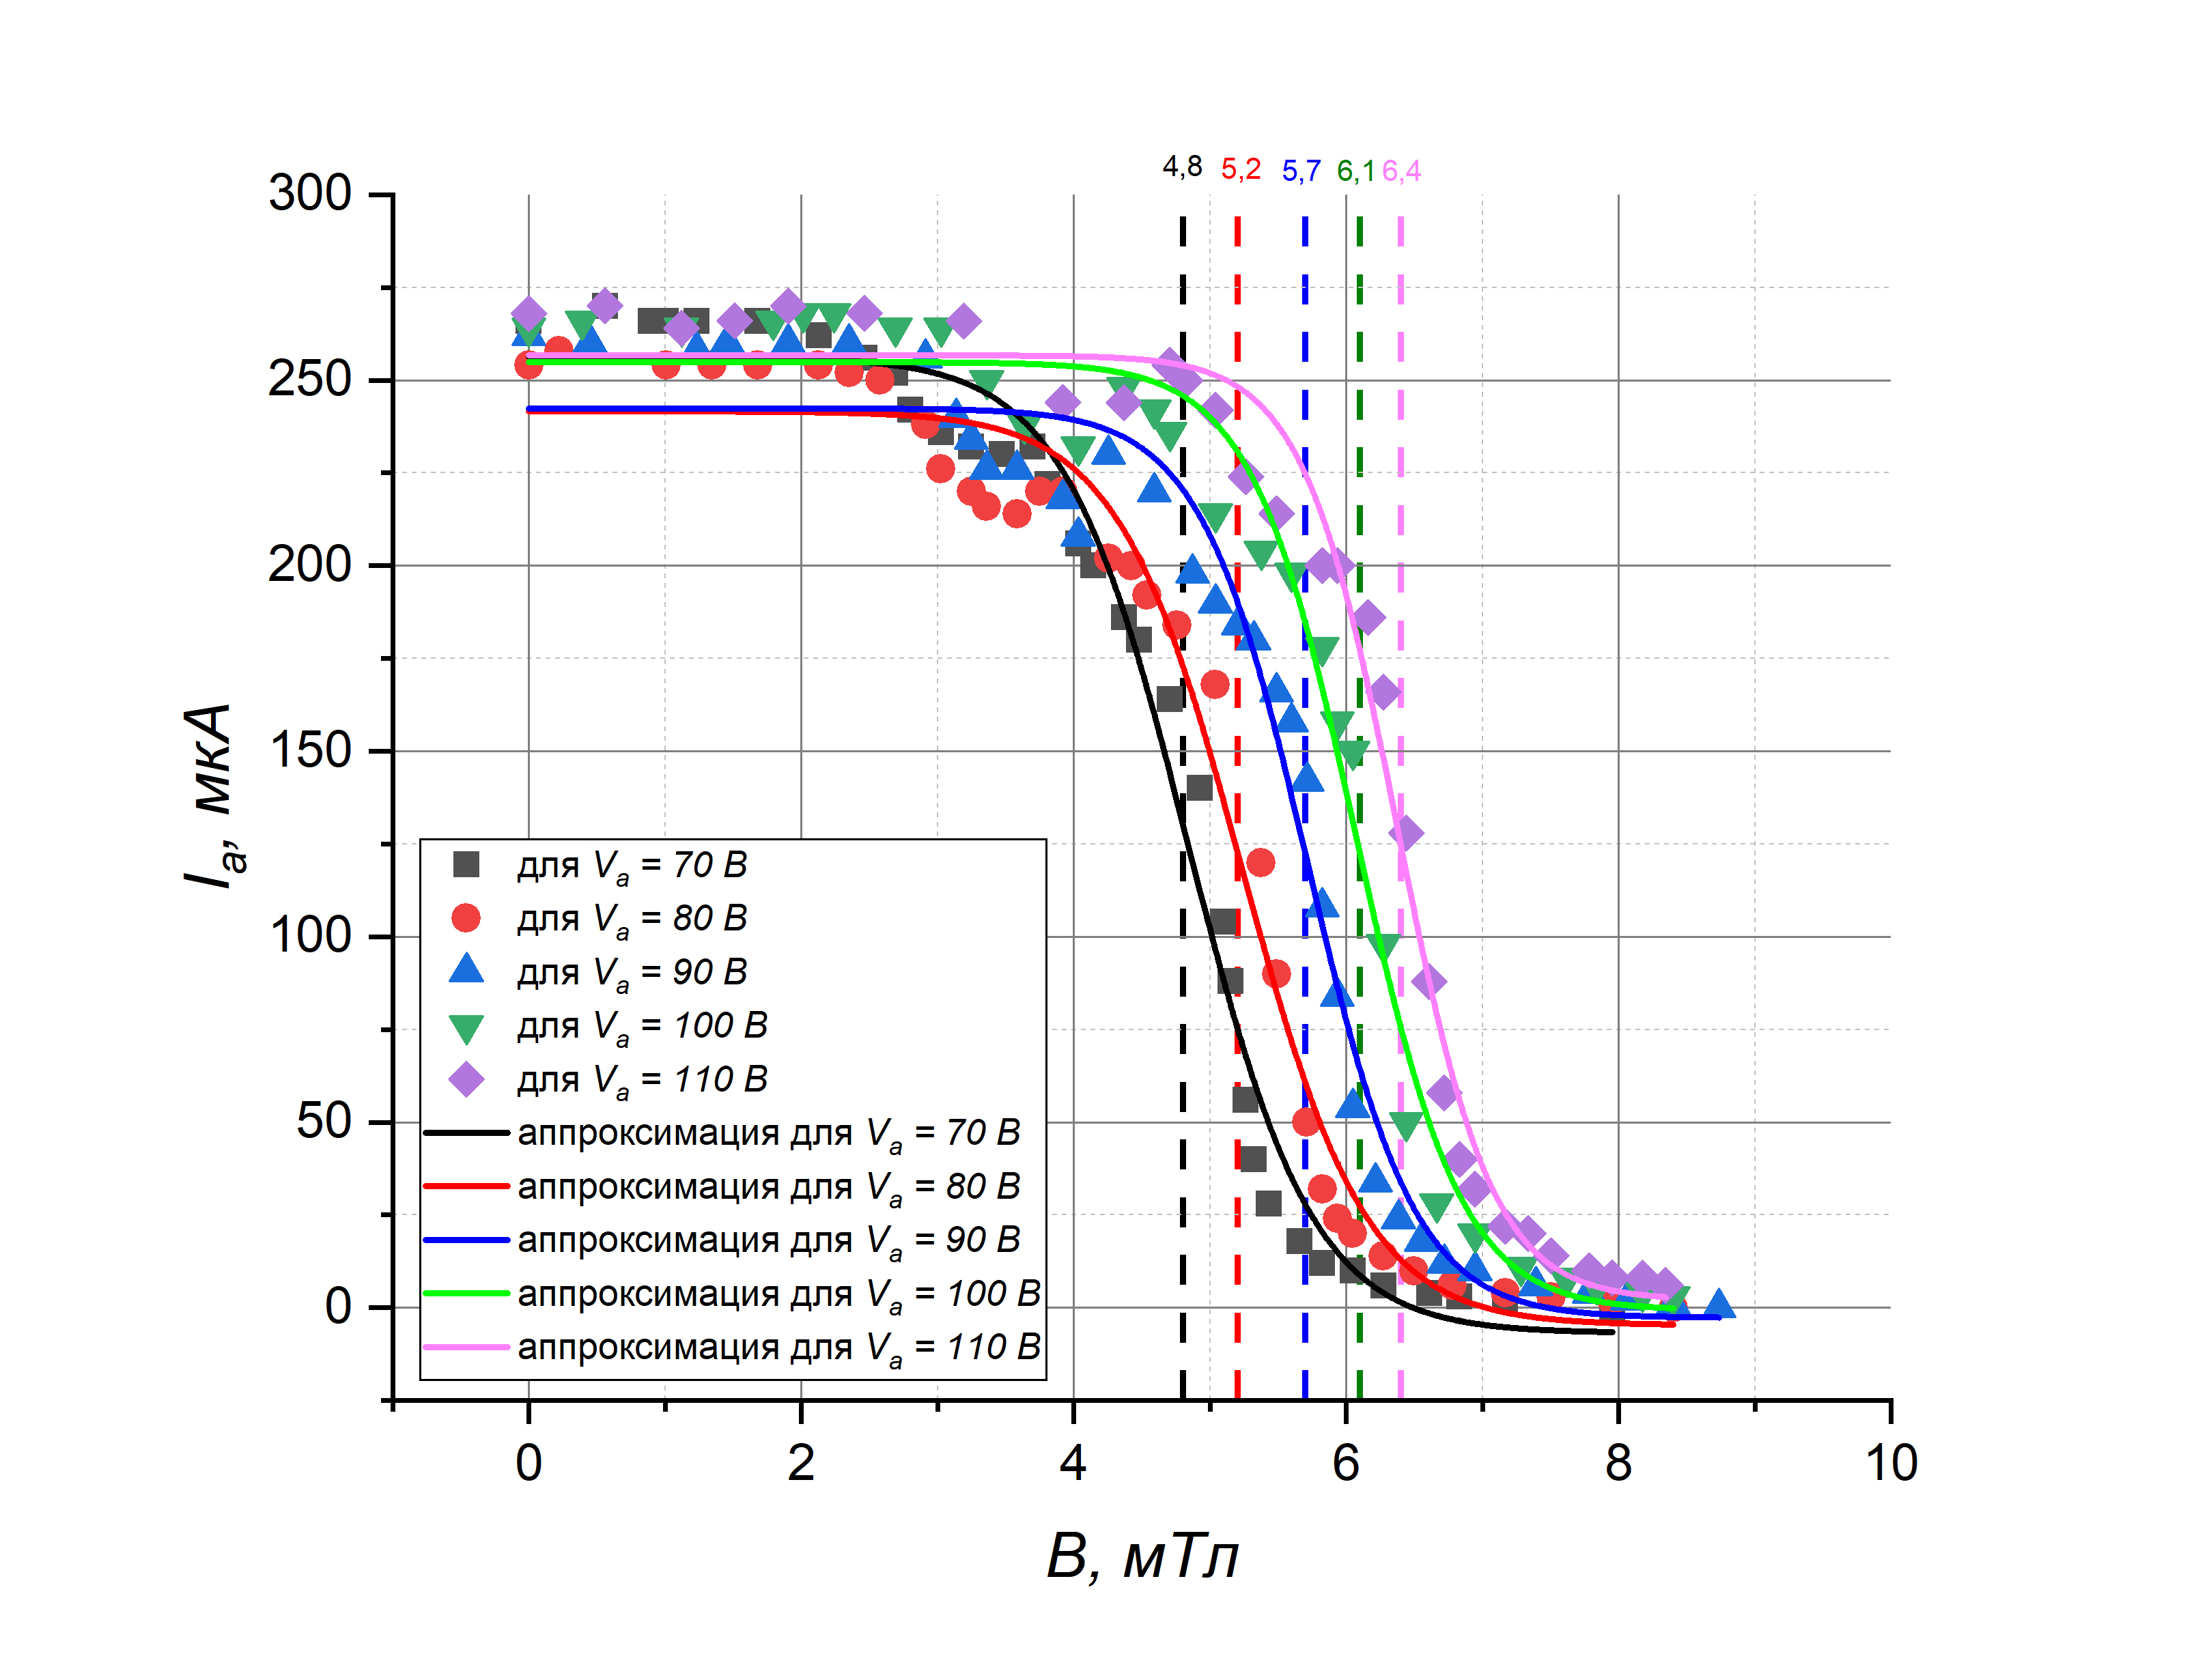
\includegraphics[width = \textwidth]{7.jpg}\\
\textbf{График 5. } График для определения $B_{\text{кр}}$ в зависимости от $V_a$.
\end{center}
По этому графику мы получаем зависимость $B_{\text{кр}}^2$ от $V_a$.
\begin{center}
\begin{tabular}{|c|c|}
\hline
$B_{\text{кр}}^2$, $\cdot 10^{-5}$ Тл$^2$ & $V_a$, В \\ \hline
2,3 & 70 \\ \hline
2,7 & 80 \\ \hline
3,25 & 90 \\ \hline
3,72 & 100 \\ \hline
4,1 & 110 \\ \hline
\end{tabular}\\
\textbf{Таблица 11.} $B_{\text{кр}}^2$ от $V_a$
\end{center}
По этим данным построим график.
\begin{center}
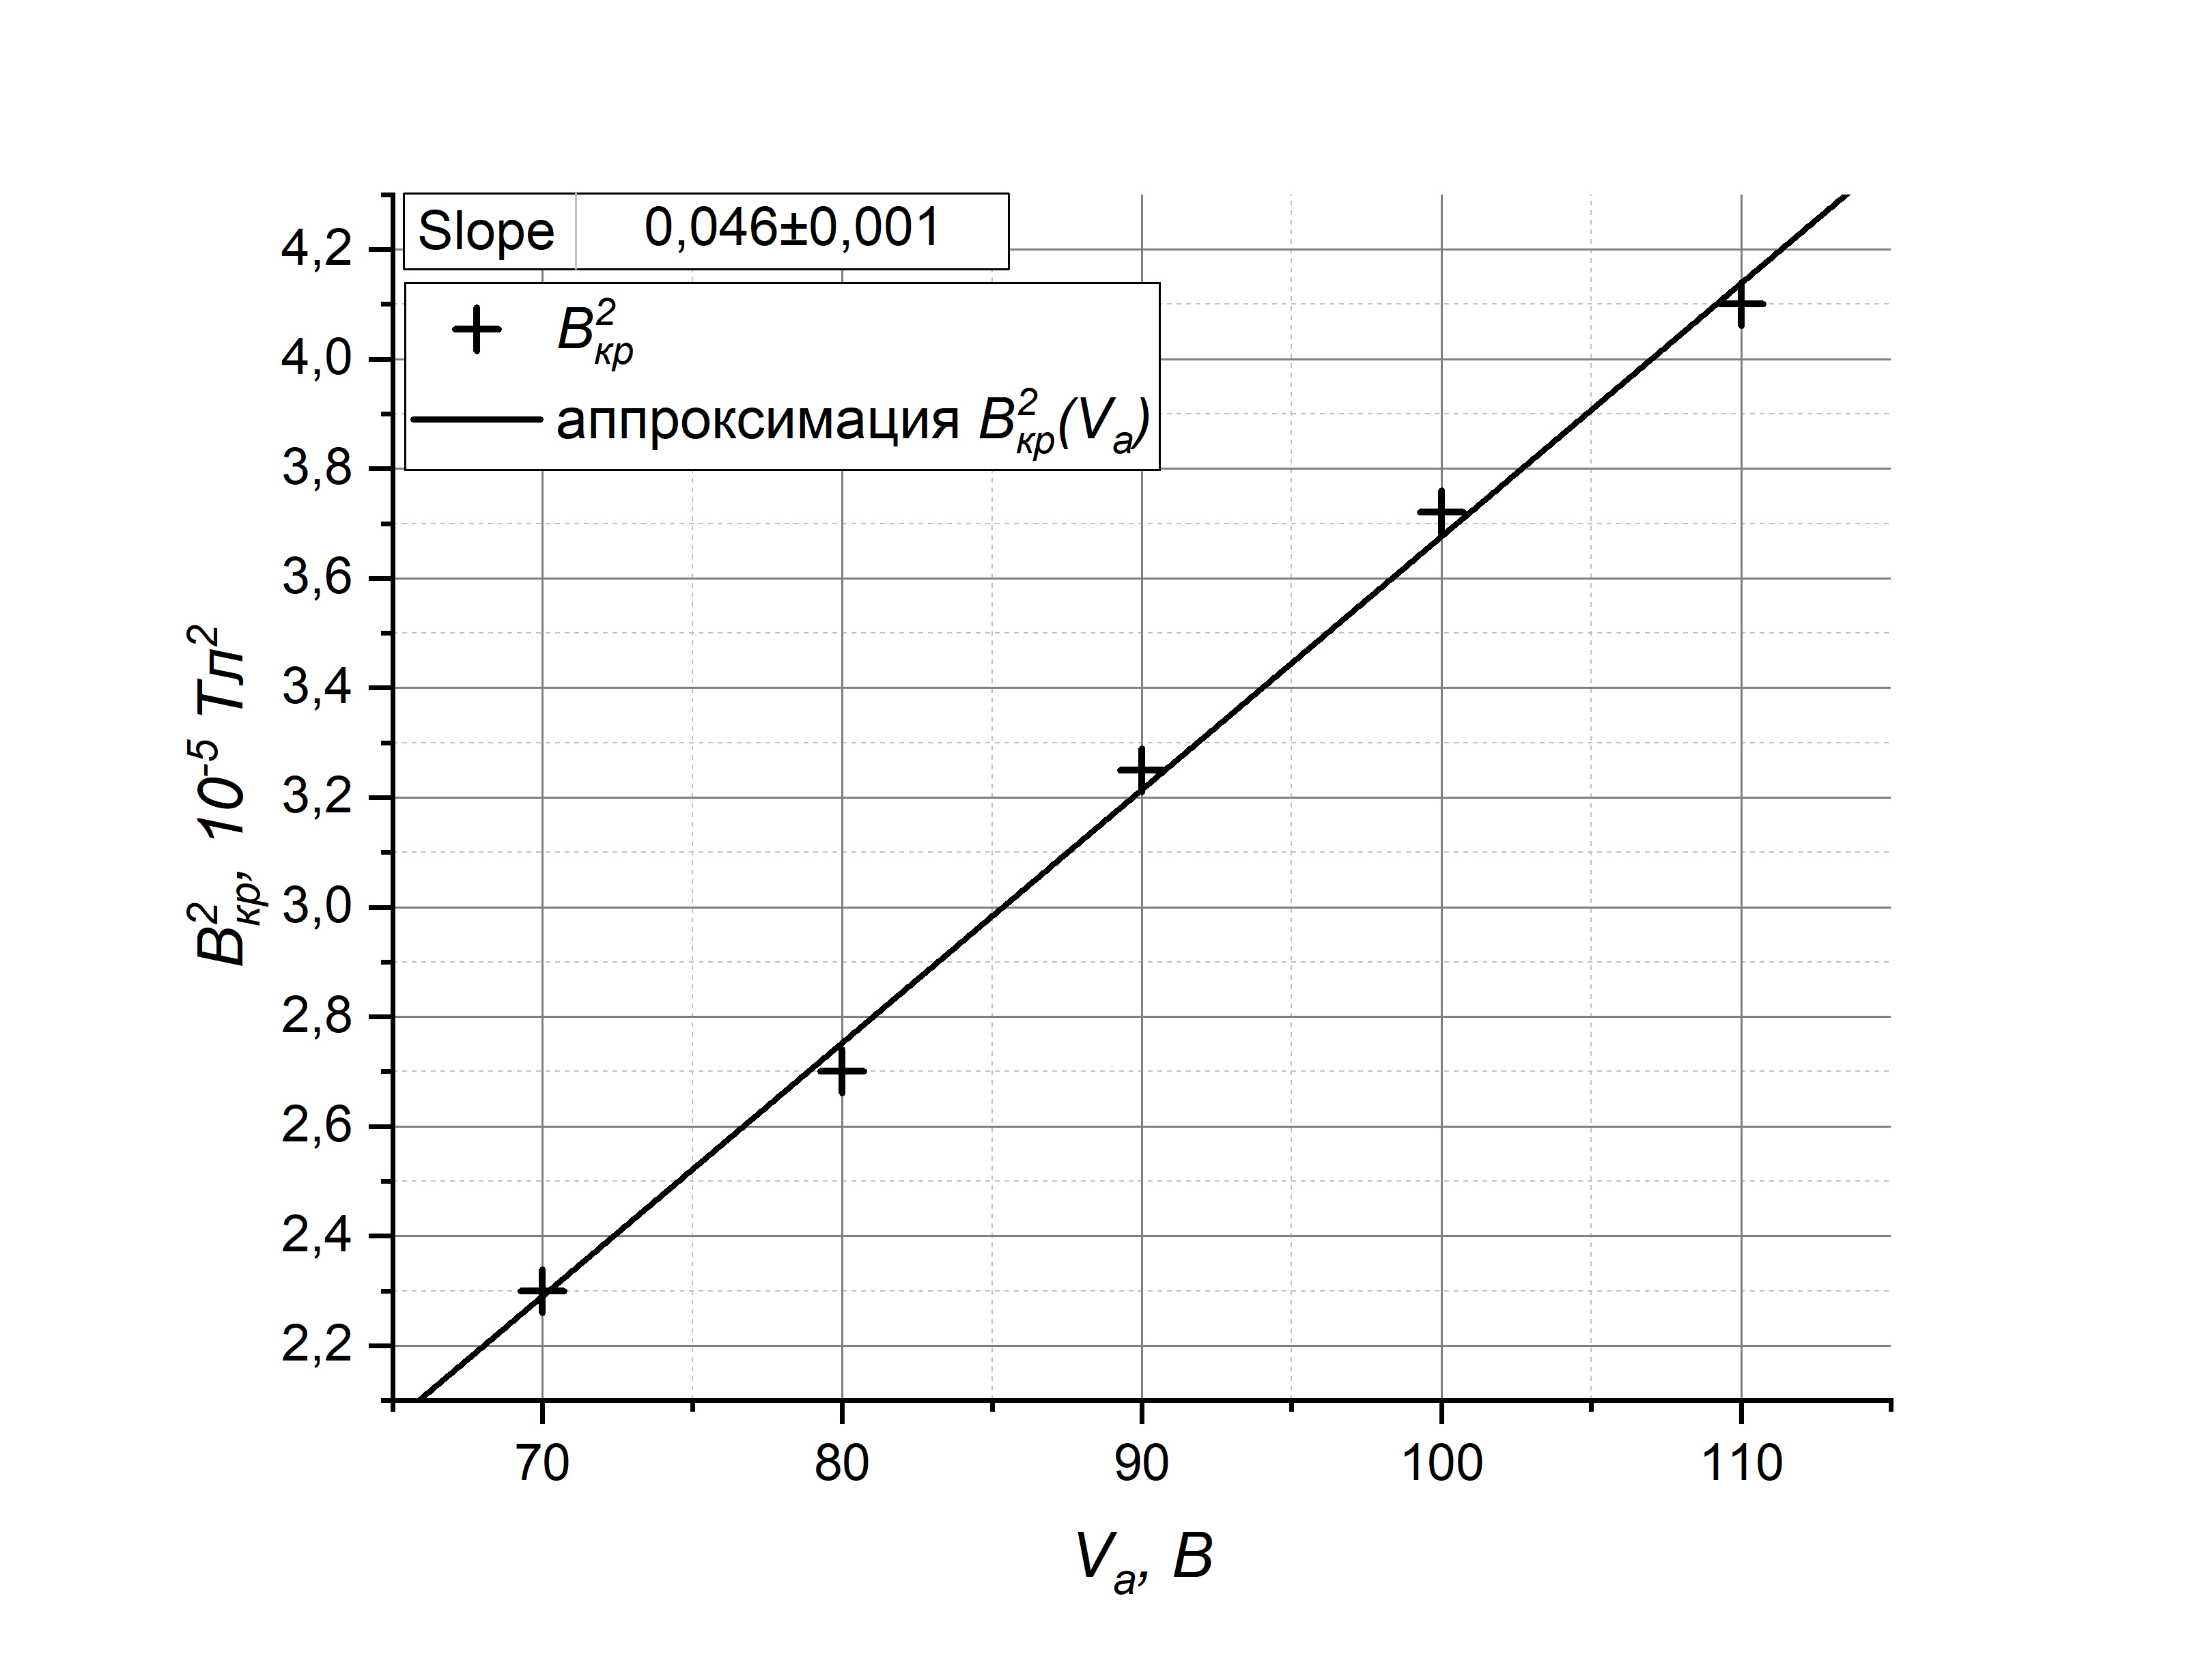
\includegraphics[width = \textwidth]{8.jpg}\\
\textbf{График 6. } График зависимости $B_{\text{кр}}^2$ от $V_a$.
\end{center}
По этим данным мы получаем 
\[\dfrac{e}{m} = (1,3 \pm 0,5) \cdot 10^{11} \text{Кл}/\text{кг}\]
Что так же близко в пределах погрешности к табличному результату.
\section*{Используемая литература.}
\begin{enumerate}
\item \textbf{Лабораторный практикум по общей физике:} Учебное пособие. В трех томах. Т. 2. Электричество и магнетизм /Гладун А.Д., Александров Д.А., Берулёва Н.С. и др.; Под ред. А.Д. Гладуна - М.: МФТИ, 2007. - 280 с.
\item \textbf{Дополнительное описание лабораторной работы 3.3.1}: Резонанс напряжений; Под ред. МФТИ, 2016 г. - 5 с.
\end{enumerate}
\end{document}
